To make sure the simulation reproduces the data, we reweight the number of
primary verteces in the simulation to match the distribution observed in the 
data, after requiring that the event has two leptons passing offline
lepton selection. The number of Primary verteces in data and simulation before and
after applying the reweighting procedure in dilepton events is shown in
Figure~\ref{fig:nvert_zll}. The weight factor applied to the simulation 
depending on the number of primary verteces is listed in 
Table~\ref{tab:nvert_zll}.

\begin{figure}[!htbp]
\begin{center}
   \subfigure[]{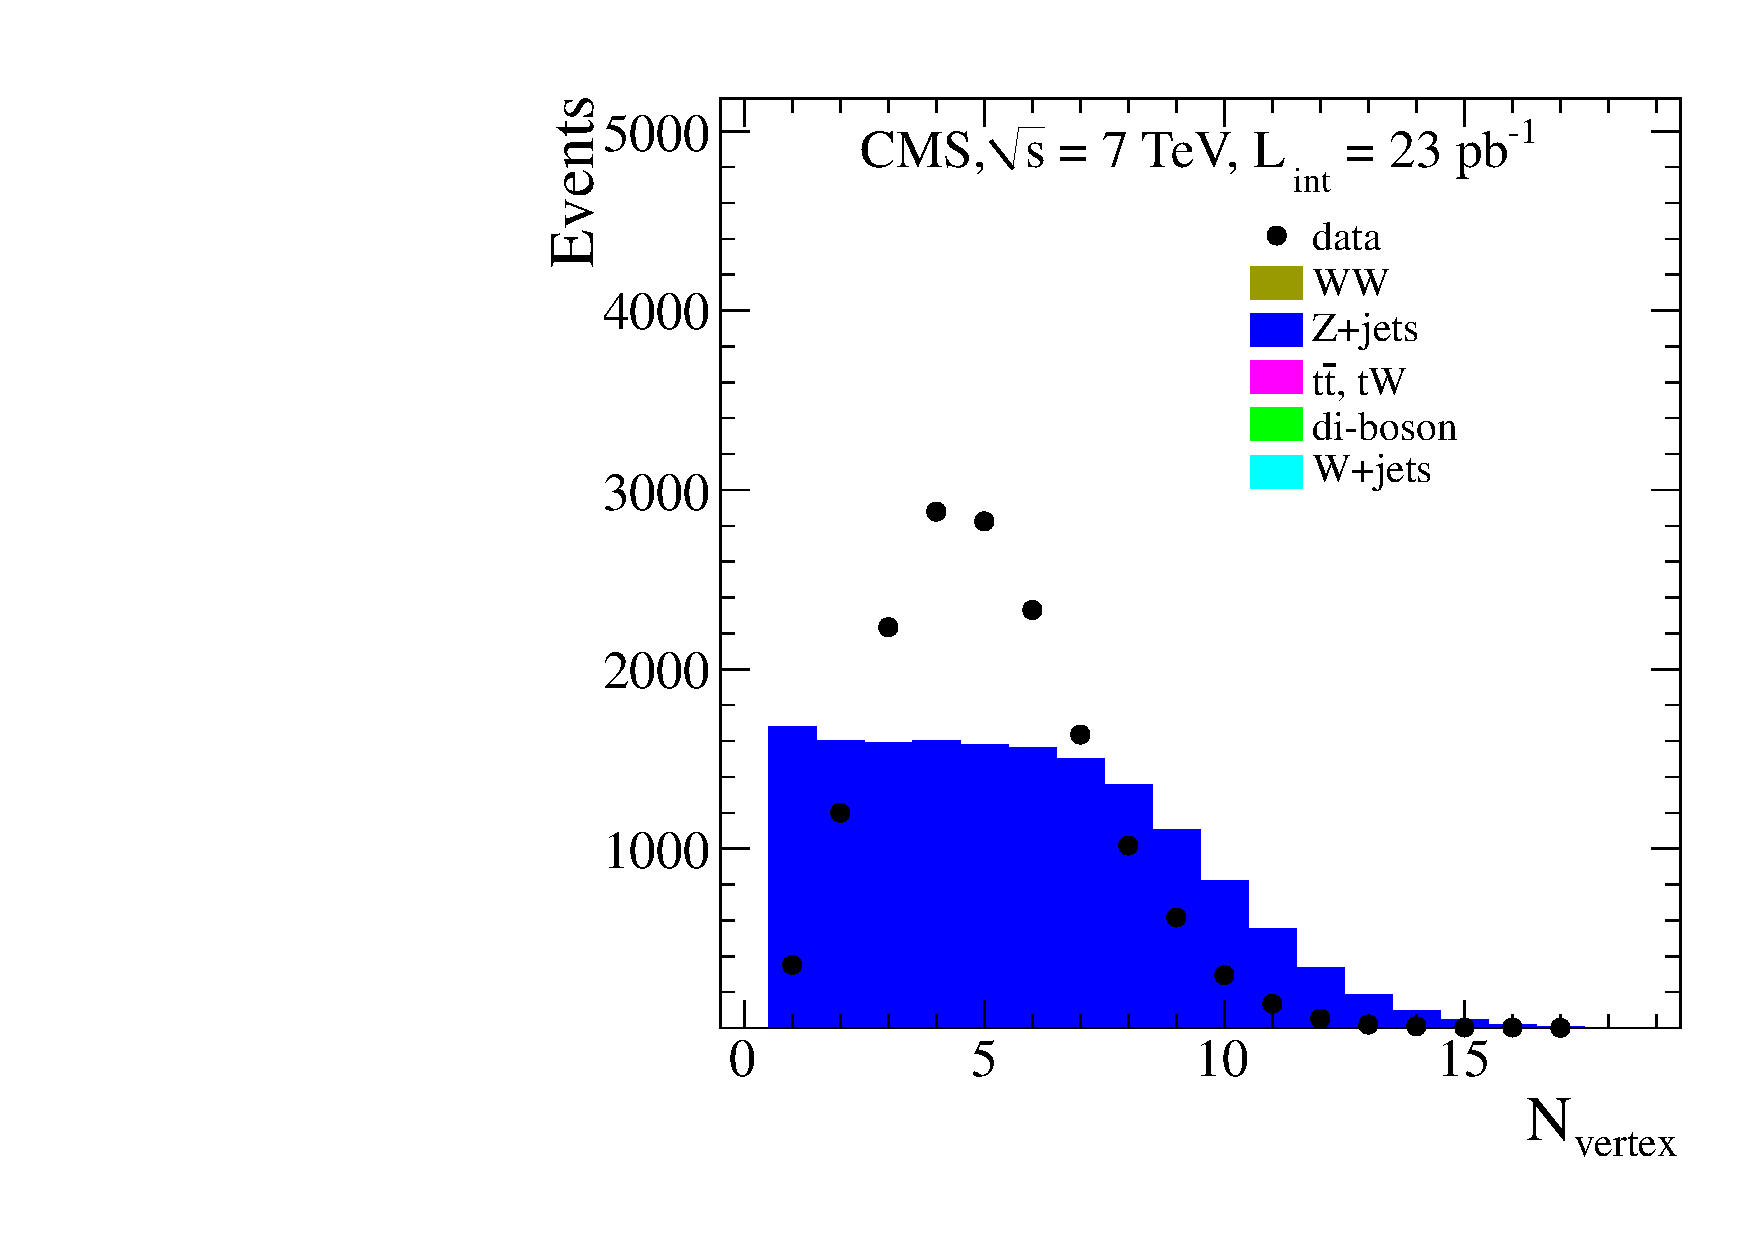
\includegraphics[width=0.49\textwidth]{figures/nvert_zll_noreweight.pdf}}
   \subfigure[]{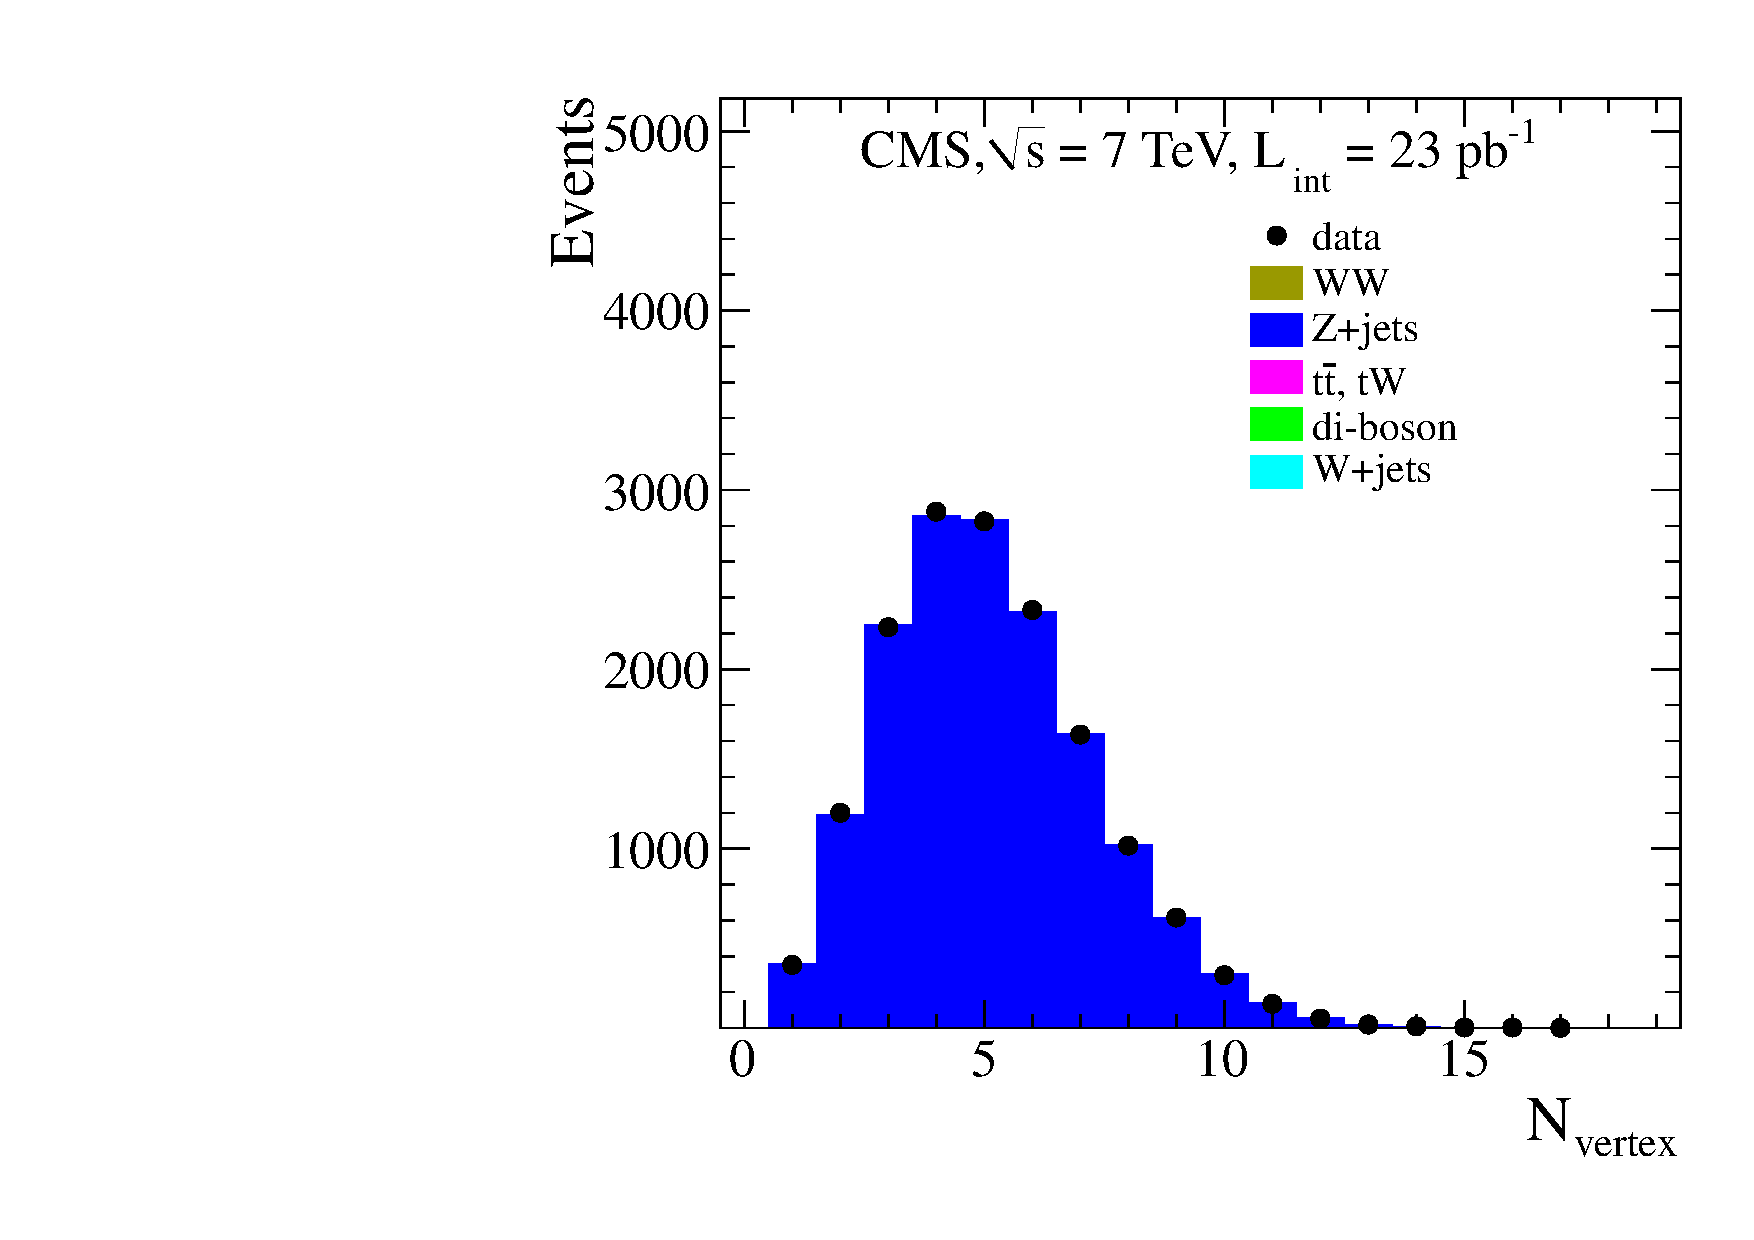
\includegraphics[width=0.49\textwidth]{figures/nvert_zll_reweight.pdf}} 
\caption{Number of Primary verteces in data and simulation before (a) and
after (b) applying the reweighting procedure in dilepton events.}
\label{fig:nvert_zll}
\end{center}
\end{figure}

\begin{table}[!ht]
\begin{center}
\begin{tabular}{|c|c|}
\hline
 $N_{vertex}$ &   weight   \\
\hline
\hline
 1        & 0.215 \\
 2        & 0.742 \\
 3        & 1.414 \\
 4        & 1.780 \\
 5        & 1.796 \\
 6        & 1.486 \\
 7        & 1.092 \\
 8        & 0.752 \\
 9        & 0.556 \\
10        & 0.369 \\
11        & 0.255 \\
12        & 0.166 \\
13        & 0.114 \\
14        & 0.106 \\
15        & 0.056 \\
$\geq$16  & 0.010 \\
\hline
\end{tabular}
\caption{Weight factor applied to the simulation depending on the number of
primary verteces.\label{tab:nvert_zll}}
\end{center}
\end{table}
